\begin{pages}
    \begin{Rightside}
    \selectlanguage{greek}
        \beginnumbering
        \pstart[
        			\chapter{Αἱ τῶν ἀγγέλων πληγαί}
        			\markboth{The Plagues of the Angels}
				]
		Καὶ εἶδον ἄλλο σημεῖον ἐν τῷ οὐρανῷ μέγα καὶ θαυμαστόν, ἀγγέλους ἑπτὰ ἔχοντας πληγὰς ἑπτὰ τὰς ἐσχάτας, ὅτι ἐν αὐταῖς ἐτελέσθη ὁ θυμὸς τοῦ Θεοῦ. Καὶ εἶδον ὡς θάλασσαν ὑαλίνην μεμιγμένην πυρί, καὶ τοὺς νικῶντας ἐκ τοῦ θηρίου καὶ ἐκ τῆς εἰκόνος αὐτοῦ καὶ ἐκ τοῦ ἀριθμοῦ τοῦ ὀνόματος αὐτοῦ ἑστῶτας ἐπὶ τὴν θάλασσαν τὴν ὑαλίνην, ἔχοντας κιθάρας τοῦ Θεοῦ. 
		\pend
		\pstart
		καὶ ᾄδουσιν τὴν ᾠδὴν Μωϋσέως τοῦ δούλου τοῦ Θεοῦ καὶ τὴν ᾠδὴν τοῦ Ἀρνίου, λέγοντες 	Μεγάλα καὶ θαυμαστὰ τὰ ἔργα σου, Κύριε ὁ Θεός ὁ Παντοκράτωρ· δίκαιαι καὶ ἀληθιναὶ αἱ ὁδοί σου, ὁ Βασιλεὺς τῶν ἐθνῶν· τίς οὐ μὴ φοβηθῇ, Κύριε, καὶ δοξάσει τὸ ὄνομά σου; ὅτι μόνος ὅσιος, ὅτι πάντα τὰ ἔθνη ἥξουσιν καὶ προσκυνήσουσιν ἐνώπιόν σου, ὅτι τὰ δικαιώματά σου ἐφανερώθησαν. 
		\pend
		\pstart
		Καὶ μετὰ ταῦτα εἶδον, καὶ ἠνοίγη ὁ ναὸς τῆς σκηνῆς τοῦ μαρτυρίου ἐν τῷ οὐρανῷ, καὶ ἐξῆλθον οἱ ἑπτὰ ἄγγελοι οἱ ἔχοντες τὰς ἑπτὰ πληγὰς ἐκ τοῦ ναοῦ, ἐνδεδυμένοι λίνον καθαρὸν λαμπρὸν καὶ περιεζωσμένοι περὶ τὰ στήθη ζώνας χρυσᾶς. καὶ ἓν ἐκ τῶν τεσσάρων ζῴων ἔδωκεν τοῖς ἑπτὰ ἀγγέλοις ἑπτὰ φιάλας χρυσᾶς γεμούσας τοῦ θυμοῦ τοῦ Θεοῦ τοῦ ζῶντος εἰς τοὺς αἰῶνας τῶν αἰώνων. καὶ ἐγεμίσθη ὁ ναὸς καπνοῦ ἐκ τῆς δόξης τοῦ Θεοῦ καὶ ἐκ τῆς δυνάμεως αὐτοῦ, καὶ οὐδεὶς ἐδύνατο εἰσελθεῖν εἰς τὸν ναὸν ἄχρι τελεσθῶσιν αἱ ἑπτὰ πληγαὶ τῶν ἑπτὰ ἀγγέλων.
		\pend
        \endnumbering
    \end{Rightside}
    \begin{Leftside}
        \beginnumbering
        \pstart[
        			\chapter{The Plagues of the Angels}
				]		
		And I saw another great and wondrous sign in Heaven: an angel having (with him?) the last seven plagues (seven last plagues), for in them the wrath of God will be finished. And I saw (something) like a crystalline (made out of glass) sea mixed with fire; and those who prevailed over the beast and over its idol and over the number of its name, (they were) standing upon the crystalline sea (each of them) having lyres of God. 
		\pend
		\pstart
		And they sing the ode (song) of Moses — the servant of God — and the ode (song) of the Lamb saying, “Great and wondrous are Your deeds, O Lord God, the Almighty. Just and true are Your ways, O King of (all) the nations. Who does not fear and glorify Your name, O Lord? For (You) alone are holy (hallowed) and because all the nations will come (to You) and worship before You and because Your righteous deeds were revealed.”
		\pend
		\pstart
		And after this I saw and the temple of the tabernacle of the testimony open in Heaven and there came out of the temple the seven angels, (namely the ones) having the seven plagues (and they were) clad in pure, white linen; and around their chests were bound golden belts. And one of the four creatures gave seven golden vials — (all) filled with the wrath of God, the (one) living into the eternity of eternity — to the angels. And the temple was filled with smoke from the glory of God and from His power; and nobody was able to enter into the temple until the seven plagues of the seven angels have finished. 
		\pend
        \endnumbering
    \end{Leftside}

\end{pages} 
\Pages

\clearpage
\thispagestyle{empty}
\null\vfill
\settowidth\longest{\huge\itshape […] and when I turned around I saw}
\begin{center}
\parbox{\longest}{%
  \raggedright{\huge\itshape%
    ``And after this I saw and the temple of the tabernacle of the testimony open in Heaven and there came out of the temple the seven angels.'' \par\bigskip
  }
  \raggedleft\Large\MakeUppercase{``Zornschalen'' — Gebhard Fugel, 1933}\par%
}
\vfill\vfill
\clearpage\newpage
\end{center}
\newpage
\thispagestyle{empty}
\begin{center}
	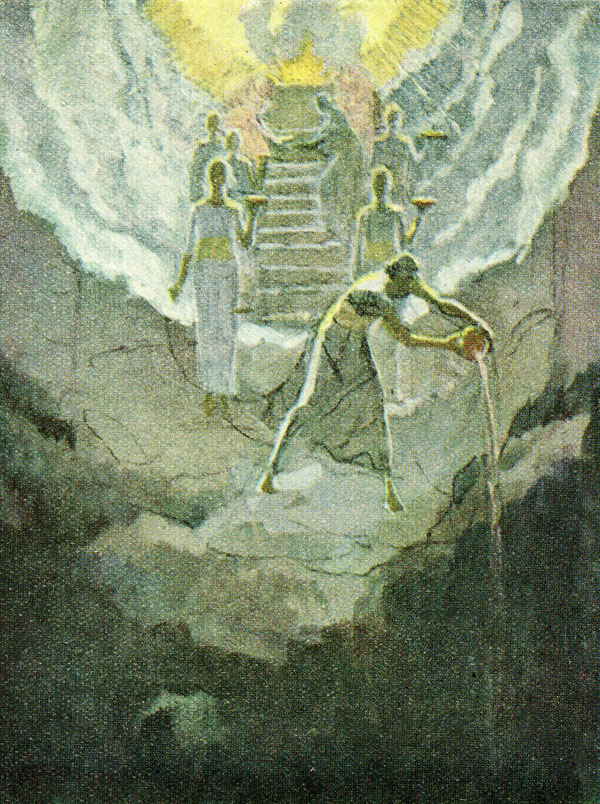
\includegraphics[width=1\textwidth]{images/illustrations/fugelzornschalen}
\end{center}